\documentclass{my_paper}
\usepackage{ctex}
\usepackage[textwidth=444bp,vmargin=2.5cm]{geometry}%设置页边距
\usepackage{array} %主要是增加列样式选项
\usepackage[dvipsnames]{xcolor}%颜色宏包
\usepackage{graphicx}%图片宏包
\usepackage{amsmath}%公式宏包
\usepackage[T1]{fontenc}    
\usepackage{newtxtext, newtxmath}  %两种使用Times New Roman 字体的方法
\usepackage{subfigure}
\usepackage{tabularx, booktabs} %% Load packages that you use
\usepackage{multirow} %跨行处理
\usepackage{rotating}%横向表格
\usepackage{diagbox}%斜线划分表头

\usepackage { gensymb }
% 打°符号\degree
\usepackage{framed}
\usepackage{listings}
% 代码
\usepackage{color} %red, green, blue, yellow, cyan, magenta, black, white
\usepackage[numbered,framed]{matlab-prettifier}%matlab 代码高亮
\usepackage{mdframed}%另一个边框
% matlab代码样式,使用方法为:
% \lstinputlisting[style=Matlab-editor,linewidth=\textwidth]{code.m}
% 或:
% \begin{lstlisting}[style=matlab-prettifier]
%     %code
% \end{lstlisting}
\renewenvironment{framed}[1][\hsize]
  {\MakeFramed{\hsize#1\advance\hsize-\width \FrameRestore}}%
  {\endMakeFramed}
%   修正framed环境,使之可以变长,用法:
%   \begin{framed}[1.2/textwidth]...

\begin{document}

\lstdefinestyle{python_style}{
 columns=fixed,
 numbers=left,                                        % 在左侧显示行号
 numberstyle=\tiny\color{gray},                       % 设定行号格式
 frame=trbl,                                        % 单线背景边框
 breaklines=true,                                     % 设定LaTeX对过长的代码行进行自动换行
 keywordstyle=\color[RGB]{40,40,255},                 % 设定关键字颜色
 numberstyle=\footnotesize\color{darkgray},
 commentstyle=\it\color[RGB]{0,96,96},                % 设置代码注释的格式
 stringstyle=\rmfamily\slshape\color[RGB]{128,0,0},   % 设置字符串格式
 showstringspaces=false,                              % 不显示字符串中的空格
 language=python,                                        % 设置语言
 basicstyle=\linespread{1.0}\fontsize{10bp}{10bp}\selectfont\ttfamily,                      % 字体字号
 %lineskip=10bp,
 %baselinestretch=1,
}
\newpage
\begin{center}
\lunwenbiaoti

\vspace{2ex}
\zhaiyao
\end{center}

摘要

\begin{guanjianci}
 元胞自动机 \quad 边缘检测 \quad 形状匹配
\end{guanjianci}

%----------- 正文 ----------
%----------- 一、问题重述 ----------
\newpage
\section{一、问题重述}

暖气在我国北方地区被广泛使用,在寒冷的气候条件下,暖气可以调节室内温度,带来舒适的室内环境。在使用暖气的过程中,人们常常希望把温度控制在舒适的范围内。因此如何通过控制供热水流的大小来调节室内温度成为广大研究者关注的问题。

一种智能温控器被用于完成调节温度的任务。这一工具具有调节流量的作用,可以主动调节水流大小,以满足升高温度的需求,对于降低温度而言,只能关闭阀门留待暖气片中的水流自然冷却,温度回落到室温。该装置存在温度调节不智能,过度加热或冷却,温度波动变化大的缺点。

经过分析整理,我们需要解决以下问题:
\begin{enumerate}
    \item 分析一个房间的采暖过程中的热量从供热管道到加热房间的过程,并建立模型来描述供热的水温与热水流量与房间内温度的关系。
    \item 在给定波动的室外温度条件下,针对室内某个位置设定的目标温度,设计对供热水流的调节方法。以尽可能少的次数来调节水流大小,使得室内温度最快达到目标温度。并利用附件中的数据给出控制的结果,说明方法的合理性。
    \item 假设温度控制器能记录下过去的调节结果,比如室外温度,用户设定温度,供热水阀门开闭程度,热水温度等。房间大小、房间中的属性、封闭程度、墙窗门的比例、墙壁保温程度等相对固定的。在上述条件下,对第二问中的控制方法进行优化。
\end{enumerate}

\section{二、问题分析}
\subsection{问题一的分析}

问题一我们需要分析房间采暖过程的热量转移过程,要求我们就暖气这一供热装置的原理有所了解。为此需要查阅资料与相关参数,分析暖气片的热交换方式,以及分析进水温度$T_{wi}$和出水温度$ T_{wo} $与热量传递$Q$之间的关系。为了建立模型,描述供热水温与热水流量同房间内温度的关系问题,需要就房间的整体结构进行分析。房间由墙体,窗户,以及天花板构成,部分墙体属于外墙与室外相接触,而有的墙体又属于内墙,内外墙之间的传热能量具有差异。此外,考虑空气导热性质不佳的特点,需要结合传热学知识,建立全屋的空气热量模型。

\subsection{问题二的分析}

针对问题二,我们需要在变化的环境温度这一条件下,动态控制热水的流入速率,使得室内温度尽可能达到要求的水平,且维持温度,使之波动保持在一定水平内。考虑到温度控制时知道当前时刻的室外温度,以及室内某处的实时温度和目标温度,我们需要控制暖水流来实时调节温度,以达到预期目标。

但是房屋温度的影响因素多样,于温度控制器而言相当于一个黑箱,并不知道其详细的工作原理。考虑使用PID自动控制的方法来自动调节温度,以达到在外界温度变化的情况下依然保持室内恒温的效果。可以利用在问题一中建立出的温度模型来模拟PID控制的情况,以判断某一组PID参数选取的优劣。在调节PID参数的过程中不可避免需要多次搜索确定最佳的参数组合,可以采取变步长法逐步减小参数的搜索范围,最终得到最优PID参数的组合,作为我们的调控结果。

\subsection{问题三的分析}


%----------- 三、模型假设 ----------
\section{三、模型假设}
%使用代码片段:、jiashe%
\begin{enumerate}
    \item 暖气管内相邻两段水柱之间不发生热量交换。
    
    \textbf{原因:}
    相邻两段水柱之间温度差较小,且表面积也小,暖气管内水流的热量散失主要是由向外界散发所导致。

    \item 建筑内墙和地板认为是绝热体。
    
    \textbf{原因:}
    这是对房屋的理想化假设,其原因为内墙两侧温差不大,因此认为没有热交换。由于地板之下可能是地基或下一层住户,也可认为温差不大不予考虑。
    
    \item 室内窗户皆处于关闭状态。
    
    \textbf{原因:}
    我国北方地区气候严寒,开窗的情况下难以保持室内温度,且开窗条件下室内外的空气流动,难以计算其热量交换数值。

    \item 室内的气压保持稳定不变。
    
    \textbf{原因:}
    虽然室内的窗户处于关闭状态,但是仍有缝隙保持气压平衡。

    \item 忽略暖气片的厚度,将其视作会发热的墙壁区域。
    
    \textbf{原因:}
    该做法有利于简化问题,利于分析屋内传热情况,且暖气片的厚度和房间进深相比较小,不构成太大影响。

\end{enumerate}

%----------- 四、符号说明 ----------
\section{四、名词解释与符号说明}
%使用三线表格最好~
\subsection{名词解释}
\begin{enumerate}
    % 名词:、mingci
    \item \textbf{dada}
    
    dsadw
    
    \item \textbf{dsadc}
    
    dasdsas

    
\end{enumerate}
\subsection{符号说明}
以下是本文使用的符号以及含义:
\begin{table}[h]%htbp表示的意思是latex会尽量满足排在前面的浮动格式,就是h-t-b-p这个顺序,让排版的效果尽量好。
    \centering
    \begin{tabular}{p{2.0cm}<{\centering}p{9.0cm}<{\centering}p{2.0cm}<{\centering}}
 %指定单元格宽度, 并且水平居中。
    \hline
    符号 & 说明 & 单位 \\ %换行 
    \hline
    $L_0$ & 仓库长度 &  $m$\\
    
    \hline
    \end{tabular}
\end{table}

%----------- 五、模型的建立与求解 ----------
\section{五、模型的建立与求解}

以下将对提出的三个问题进行建模求解。
\subsection{热水调控的房间温度模型}

为了解决问题一,我们提出一种以房间热水流量和热水温度为输入,以最终房屋每处温度随时间的变化为输出的模型。为此,我们对暖气片的工作原理,房间的结构和传热特性进行分析。在得到房屋的热量传递模型后,结合牛顿冷却定律、傅里叶传热定律以及热量守恒定律,建立离散化的屋内温度模型。

\subsubsection{暖气片供热模型}

暖气片利用热水在管中流动的过程,加热其周围的空气,并传递热量到周围,是一种典型的间壁式散热器\cite{2}。在工作过程中,暖气片的热水从一端流入,并且从另一端流出较冷的水,在内部为相连的若干U形管相连,如 图(\ref{nuanqipian})所示:

\begin {figure}[h]
\centering % 居中显示
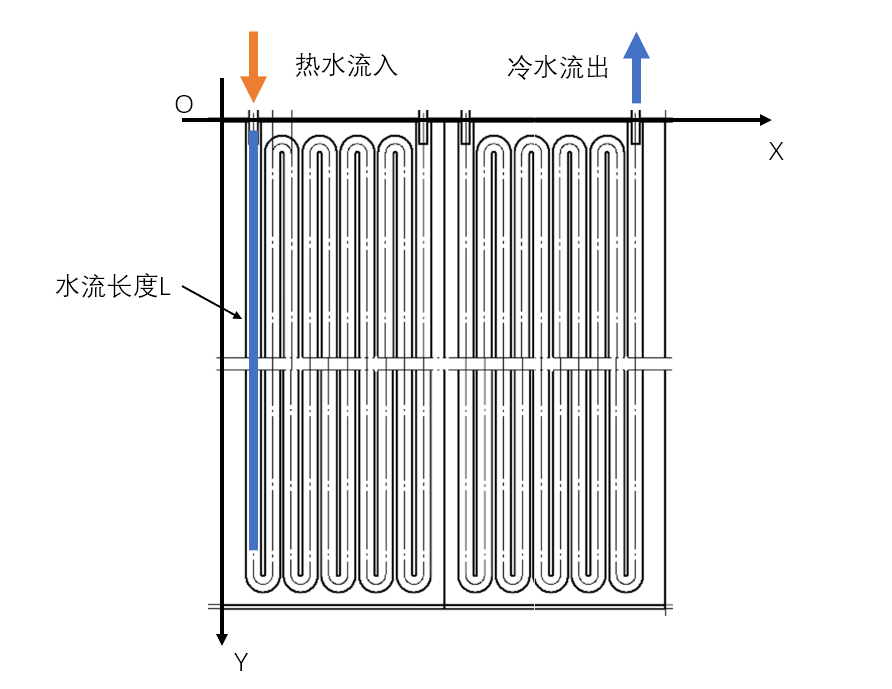
\includegraphics[width=\textwidth]{nuanqipian.png}
说明:为展示方便,z轴垂直纸面向内,隐去不画。
\caption{暖气片内部水流示意图} % 标题
\label{nuanqipian}
\end {figure}

在$ t=0 $时,热水还未流入管内,此时管内水流温度等于室内温度$ T $;

在经过时间 $t_0$ 后,热水流入管中,此时管中热水长度$l$为:

\begin{equation}
l_0 = \int^{t_0}_{0}\frac{v(t)}{S}dt
\end{equation}

其中$ v(t) $为热水流量,随调节过程随时间变化,$ S $为暖气管的横截面积。在水流长度为$ l $的情况下,对应在图(\ref{nuanqipian})中的直角坐标系,有唯一的坐标表示$(x,y,z)=f(l)$,即:

\begin{equation}
\begin{cases}
    x = f_x(l)\\
    y = f_y(l)\\
    z = f_z(l)\\
\end{cases}
\end{equation}

取时间微元$ t\to t+dt $进行分析,此时长度变化为$dl$,使用水流速度$v(t)$,横截面积$S$计算而出。

\begin{equation}
    dl = \frac{v(t)*dt}{S}
\end{equation}

考虑该段微元处的管道导热影响,我们画出其截面图(图\ref{jiemian}),对于该段柱体而言,可以假设管内的温度为$T_1$而管外温度为$T_2$,观察暖气管的物理结构可知,满足长度远远大于其直径,可以看作是等温面共轴。在这一条件下,建立热传导微分方程:

\begin{equation}
\frac{d^{2}T}{dr^{2}} + \frac{1}{r}\frac{dT}{dr}=0
\end{equation}

使用变量代换法,将上式变形:
\begin{equation}
u = \frac{dT}{dr} \Rightarrow  \frac{du}{dr}=\frac{d^2T}{dr^2}
\label{}
\end{equation}

之后将原始微分方程变化为以下形式:
\begin{equation}
\frac{du}{dr}+\frac{u}{r} = 0
\label{}
\end{equation}

可以通过分离变量法和两部积分法,可以求出对数形式的同届:
\begin{equation}
    \begin{cases}
        ln u +lnr = lnC_1\\
        T(r) = C_1 lnr + C_2
    \end{cases}
\label{}
\end{equation}

通过给定第一类边界条件\cite{1},即表面温度分布,如下所示:
\begin{equation}
    \begin{cases}
        r = r_1 , & T = T_1\\
        r = r_2 , & T = T_2
    \end{cases}
\end{equation}

可以计算出柱体内的最终温度场形式:
\begin{equation}
    T(r) = T_1 - (T_1-T_2)\frac{lnr - lnr_1}{lnr_2 - lnr_1}
\end{equation}

利用傅里叶传热定律计算出表面的热流密度$\phi$:

\begin{equation}
    \phi = -\lambda \frac{dT}{dr} = \frac{\lambda}{r}\frac{T_1-T_2}{lnr_1-lnr_2}
\end{equation}

经过上述分析,我们建立了水流经由暖气管向外散发热量的过程,在完成上述过程后分析一段微元$dl$处的热交换情况。由于微元处的长度很小,该段微元的温度可以由微元开始处的温度$T_n(l,t_0)$所确定。我们利用牛顿冷却定律\cite{1},在水柱微元和空气之间建立如下所示的传热关系:

\begin{equation}
    \begin{aligned}
        q&= k_0*(T(x,y,z,t_0)-T_n(l,t_0))\\
        &= k_0 * (T(f_x(l),f_y(l),f_z(l),t_0)-T_n(l,t_0))
    \end{aligned}
    \label{11}
\end{equation}

其中$T,T_n$分别代表室内空气温度和暖气温度,$q$代表热流密度,含义是单位时间内单位面积处发出或接受的热量。$k_0$ 是综合传热系数,将会在求解过程中给出。我们利用$ q $可以求得一段水柱微元内的热量变化$dQ$,以及由于热量变化所导致的温度变化$dT_n$:
\begin{equation}
    \begin{aligned}
        dQ &= q* C * dl * dt\\
        &= q* C * v * dt^2
    \end{aligned}
    \label{12}
\end{equation}

$q$代表热流密度,$C$为暖气管的截面周长,$v$为热水管的流速,又依据比热容的计算公式,算出一段水柱的温度变化:
\begin{equation}
    dT_n(l,t_0) = \frac{dQ}{c*s*dl*\rho}
    \label{dt}
\end{equation}

在这里$c$代表水的比热容,$S$代表管道截面积。由于水管中水流不断移动,相邻两段微元之间的温度差很小,近似认为不发生热交换,故在我们的模型中,该暖水微元的温度变化数值$dT$为后一时刻的同一段水柱温度变化,因此式(\ref{dt})被解释为:
\begin{equation}
dT_n(l,t_0) = T_n(l+dl,t_0+dt) - T_n(l,t_0)
\label{14}
\end{equation}

也就是说在$ dt $的时间间隔内,暖水微元移动了$dl$距离,但是在分析温差变化时,还是计算同一段水柱的变化数值。至此,我们已经阐述了流水在暖气管道中的热交换问题,在下面的内容中,我们将同样使用微分的方法,以能量守恒定律,牛顿冷却定律,傅里叶传热定律建立屋内空气变化模型。

\subsubsection{房屋的传热学分析}

对于一间房屋而言,其内部空气的温度受到墙壁种类,开窗的情况,以及天花板与外界的接触情况影响,我们将对这些因素逐一进行分析。
\begin{enumerate}
    \item 对墙面的分析
    
    注意到墙面依据所处的位置被分为内墙和外墙\cite{3},划分的依据在于是否和室外空间相接触,我们将与室外空间接触的墙体视作为外墙,而不接触的称为内墙。对于外墙而言,外侧同室外的冷空气直接接触,造成温度较低,即使墙体具有部分阻隔冷气的作用,仍然会导致室内的墙体温度较低,带走室内的空气热量。对于内墙而言,内墙两侧都是室内空气,温度差值不大,可以近似认为内墙时绝热的,不会传导室内空气热量。
    \item 对窗户的分析
    
    外墙上常常装有窗户,与外界空气联通,因此会带来室内的空气交换与热量传递。即使是在没有打开窗户的情况下,热量交换也会透过玻璃进行。在分析房内温度的过程中,也应当对窗户加以考虑。
    \item 对天花板和地面的分析
    
    对于天花板而言,其与外界直接接触,本质同外墙没有区别,会向屋外散发热量。而分析可知地面温度随气温的变化程度较之于大气变化速度较慢,且有地基等因素的存在,确定地面的温度变化较为困难,因此将其认为绝热。
    

\end{enumerate}

综合上述分析,我们对给定的矩形房屋建模,建立直角坐标系,标注其内外墙面的顶点坐标和对应类别,并以坐标形式呈现:

\begin{equation}
    \begin{aligned}
        \text{内墙:}&(x_{11},y_{11},z_{11})&(x_{12},y_{12},z_{12})\\
                    &(x_{13},y_{13},z_{13})&(x_{14},y_{14},z_{14})\\
                    &(x_{21},y_{21},z_{21})&\cdots \\
        \text{外墙:}&(x_{11},y_{11},z_{11})&(x_{12},y_{12},z_{12})\\
        &(x_{13},y_{13},z_{13})&(x_{14},y_{14},z_{14})\\
        &(x_{21},y_{21},z_{21})&\cdots \\
        \text{窗户:}&(x_{11},y_{11},z_{11})&(x_{12},y_{12},z_{12})\\
        &(x_{13},y_{13},z_{13})&(x_{14},y_{14},z_{14})\\
        &(x_{21},y_{21},z_{21})&\cdots \\
        \text{天花板:}&(x_{11},y_{11},z_{11})&(x_{12},y_{12},z_{12})\\
        &(x_{13},y_{13},z_{13})&(x_{14},y_{14},z_{14})\\
        \text{地面:}&(x_{11},y_{11},z_{11})&(x_{12},y_{12},z_{12})\\
        &(x_{13},y_{13},z_{13})&(x_{14},y_{14},z_{14})\\
    \end{aligned}
    \label{fw}
\end{equation}

可以注意到,在房屋内的空气可以进行分析,对于那些直接同外壁接触的空气微元可能发生外部的热交换,而没有同外壁接触的空气微元则只进行空气微元的交换行为,这为我们分析空气传热问题提供了有利条件。

为了分析墙壁和玻璃窗的散热速率,我们计算其传热系数$K$\cite{1},其计算公式如下:

\begin{equation}
    \large K = \frac{1}{\frac{1}{h_1}+\frac{\sigma}{\lambda}+\frac{1}{h_2}}
    \label{16}
\end{equation}

其中$h_1$和$ h_2 $是材料的热交换系数,$ \sigma $是裁量的厚度,$ \lambda $是材料的导热系数,依据这一公式可以求解出每平方米墙面或玻璃传递热量能力的大小。$K$的量纲为$W/m^2\cdot K \cdot s$,含义为单位时间内单位面积在内外相差1$K$(开尔文温度)时,传递热量的多少。利用上式可以推知,墙体(或窗户)和外界温度差为$\Delta T$时,其热流密度为:
\begin{equation}
    q = K * \Delta T
    \label{17}
\end{equation}
\subsubsection{室内空气传热模型建立}
\begin {figure}[h]
\centering % 居中显示
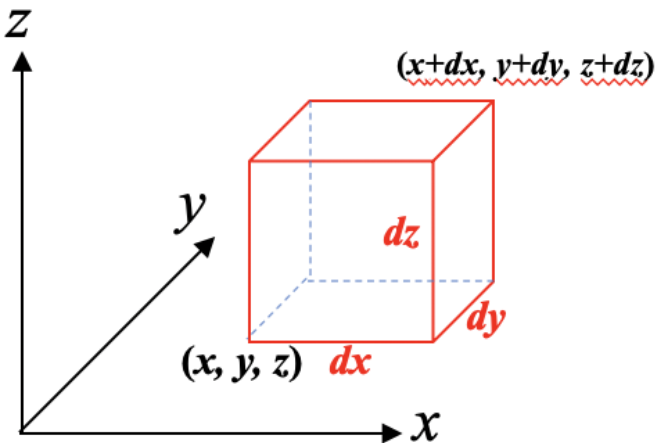
\includegraphics[width=0.7\textwidth]{weiyuan.png}
\caption{气体微元示意图} % 标题
\label{weiyuan}
\end {figure}
在分析暖气片的工作原理以及房屋的传热分析后,我们就室内的空气进行传热分析,首先利用房屋中所建立的坐标系,分析在室内空气微元$dV$中的变化过程,其中$dV$表达如下,示意图如图(\ref{weiyuan})。
\begin{equation}
dV = [(x,y,z),(x+dx,y+dy,z+dz)]
\label{}
\end{equation}

在时间间隔$[t,t+dt]$内,任何一个气体微元都满足能量守恒原理,该定理描述为微元内的能量改变只取决于传入传出能量的多少。在不考虑空气膨胀对外做功的情形,空气微元内能的变化直接反映在温度的变化上。综合以上分析,我们得出以下表达式:

\begin{equation}
    \begin{aligned}
        Q_{in} - Q_{out} = \Delta Q\\
\end{aligned}
\label{mianq}
\end{equation}

上式反映了气体微元内能变化,所带来的气体温度变化的关系,在此基础上,我们需要探究热量从高处向低处进行流动的过程,为此运用傅里叶传热定律\cite{2},用于描述相邻热量的移动多少以及对应的传热率。

\begin{equation}
    \vec{q} = -k\nabla T =\begin{cases}
        q_x = -k \frac{\partial T}{\partial  x}\\
        q_y = -k \frac{\partial T}{\partial  y}\\
        q_z = -k \frac{\partial T}{\partial  z}\\
    \end{cases} 
\end{equation}

$ \vec{q} $为热流密度矢量,表示单位时间内沿单位面积的法向流出的热量。利用上式对微元左右、前后、上下三个方向的热量变化情况进行研究,得到下式:
\begin{equation}
    \begin{aligned}
        Q_{\text{左右}} = k\frac{\partial^2 T}{\partial x^2} dtdV\\
        Q_{\text{前后}} = k\frac{\partial^2 T}{\partial y^2} dtdV\\
        Q_{\text{上下}} = k\frac{\partial^2 T}{\partial z^2} dtdV\\
    \end{aligned}
    \label{zy}
\end{equation}

考虑方向性,将式(\ref{zy})中相加整理,即得到微元流入热量$Q$:

\begin{equation}
    Q_{in}-Q_{out} = Q_{\text{左右}}+Q_{\text{前后}}+Q_{\text{上下}} = k\cdot \nabla^2 T dtdV
\end{equation}

随后将$\Delta Q$写为关于温度变化的形式:
\begin{equation}
    \begin{aligned}
        \Delta Q &= c_p * \rho * dV * [T(t+dt,x,y,z)-T(t,z,y,z)]\\
        &=c\rho \frac{\partial T}{\partial t}dtdV
    \end{aligned}
    \label{23}
\end{equation}

结合式(\ref{mianq}),我们得到热量传递关于温度变化的公式:

\begin{equation}
    k\cdot \nabla^2 T dtdV = c\rho \frac{\partial T}{\partial t}dtdV
\label{}
\end{equation}

在完成上述理论分析后,我们将对空气微元在房屋中的不同情况进行考虑,在空气微元处于房屋的内部,即微元相接触的仍然是空气,在这一情况可以认为微元在相邻的空气微元之间进行热交换,没有额外的热源进行吸放热。

而在房屋内侧边界处,也就是在式(\ref{fw})中标注的坐标范围内,空气微元在同相邻微元进行热交换的同时,还受到边界的影响而从外部热源吸热和放热。这些热源包括放热的暖气片,吸热的外墙,窗户以及天花板,以及隔绝温度交换的内墙和地面。

我们利用5.1.1中的式(\ref{11})与式(\ref{14})分别描述了暖气片微元同空气之间的热流密度$q$,以及微元处温度变化同时间$t$和空间$l$的变化关系。根据5.1.2中吸热的外墙等进行分析,我们使用式(\ref{16},\ref{17})进行计算。


借鉴有限元\cite{4}的分析思想,房屋空气任意时刻的温度分布函数$T = f(x,y,z,t)$应当是一个连续的函数,但在热源房屋这一复杂情况下,难以求解其表达式。因此将室内空气划分为在房屋内部的单元,单元形状为长宽各为$[dx,dy,dz]$的正六面体,如图(\ref{kongqiweiyuan})所示。


首先就房屋内部的微元进行分析,对于图(\ref{wya}),其热量转移方程(式\ref{23})中的偏微分方程可以写作六个方向上的差分方程,在满足能量守恒定律的条件下,计算了空气单元处的温度变化:

\begin {figure}[h]
\centering % 居中显示
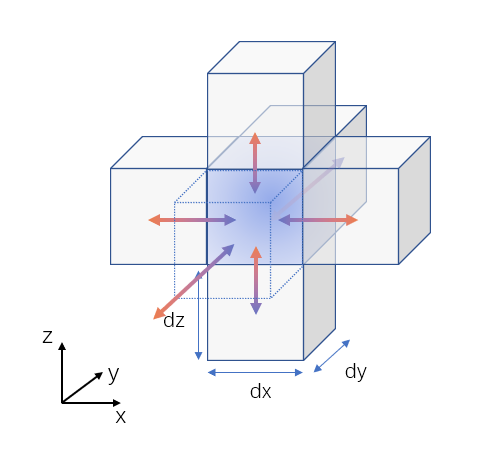
\includegraphics[width=0.7\textwidth]{wya.png}
\caption{室内微元分析} % 标题
\label{wya}
\end {figure}

\begin{equation}
        \begin{cases}
            Q_{x+} = k \cdot (T(x+dx,y,z,t)-T(z,y,z,t))dydzdt\\
            Q_{x-} = k \cdot (T(x-dx,y,z,t)-T(z,y,z,t))dydzdt\\
            Q_{y+} = k \cdot (T(x,y+dy,z,t)-T(z,y,z,t))dxdzdt\\
            Q_{y-} = k \cdot (T(x,y-dy,z,t)-T(z,y,z,t))dxdzdt\\
            Q_{z+} = k \cdot (T(x,y,z+dz,t)-T(z,y,z,t))dxdydt\\
            Q_{z-} = k \cdot (T(x,y,z-dz,t)-T(z,y,z,t))dxdydt\\
        \end{cases}
        \label{chafenw}
\end{equation}

对式(\ref{chafenw})进行整理,求解微元周围处热量变化综合求得任意一处微元在时间$[t,t+dt]$下的热量变化:
\begin{equation}
    \begin{aligned}
        \Delta Q(x,y,z,t) = k \cdot (\sum_{i\in c}T_i-6*T(x,y,z,t))*a^2*dt\\
        c = \{x+,x-,y+,y-,z+,z-\}
    \end{aligned}
\label{shi1}
\end{equation}

热量变化时,微元对应的温度变化情况为:

\begin{equation}
    \begin{aligned}
        \Delta T(x,y,z,t) &= \frac{\Delta Q(x,y,z,t)}{c_p * \rho * a^3}\\
        & = k \cdot \frac{(\sum_{i\in c}T_i-6*T(x,y,z,t))*dt}{c_p * \rho * a}
    \end{aligned}
    \label{wdjs}
\end{equation}

综合上述过程,我们已经得出内部单元的温度变化情况,其热量传递和温度变化的过程又周围六个面的微元决定。

\newpage
在分析完毕内部单元后,就和房屋边界处单元进行分析,房屋边界处单元示意图如下所示:
\begin {figure}[h]
\centering % 居中显示
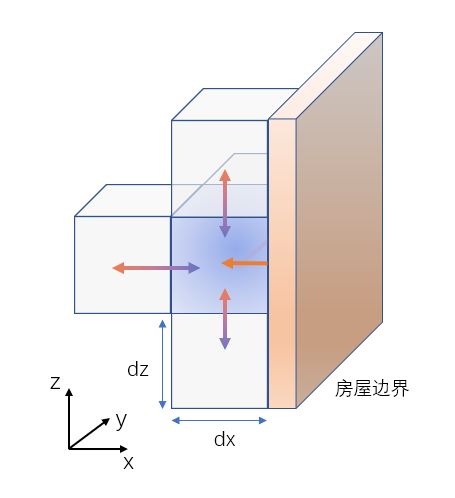
\includegraphics[width=0.7\textwidth]{wyb.png}
\caption{房屋边界处空气单元示意图} % 标题
\label{five}
\end {figure}

外部单元在空间分布上处于式(\ref{15})划定的边界范围内,因此每个边界单元至少有一面不与空气接触,但是可能随着接触外壁种类的不同而发生不同的热交换行为,具体表现在接触面的热流密度$q$上,而在其余与空气接触的面中,热转移过程仍然满足式(\ref{chafenw})中的部分规则。我们总结热量转移式如下:
\begin{equation}
    \begin{aligned}
        \Delta Q(x,y,z,t) = [k \cdot (\sum_{i\in c-c'}T_i-|c'|*T(x,y,z,t))+\sum_{i\in c'}q_i]*a^2*dt\\
        c = \{x+,x-,y+,y-,z+,z-\},c'\text{代表与房屋边界接触的单元面}
    \end{aligned}
\label{}
\end{equation}

其中$q$的取值根据边界分别为吸热边界(外墙,玻璃),绝热(地面,内墙),以及放热边界(暖气片)所决定,表述为下式:
\begin{equation}
    q = \begin{cases}
         k_0 * (T(f_x(l),f_y(l),f_z(l),t_0)-T_n(l,t_0)),& \text{放热边界}\\
         0,& ,\text{绝热边界}\\
        \Delta T \cdot \frac{1}{\frac{1}{h_1}+\frac{\sigma}{\lambda}+\frac{1}{h_2}}&,\text{吸热边界}\\
    \end{cases}
    \label{shi2}
\end{equation}

边界单元的温度变化计算公式与内部相同,由式(\ref{wdjs})给出。综合上述分析,我们已经建立了房屋内各个部分的空气单元的热量温度模型。要得出在任意时刻房间内任意地点的温度,需要在确定边界条件的情况下,模拟房间整体的传热过程,进行迭代计算。我们描述迭代计算的步骤如下,具体的计算结果,将在下一小节中给出。
{
    \renewcommand\theenumi{\chinese{enumi}}
    % 规定数字格式为罗马数字
    \renewcommand\labelenumi{\textbf{步骤\theenumi:}}
    % 规定是附录某某
    \begin{framed}[0.7\textwidth]
        \centering
        \begin{minipage}[h][0.9\textwidth][c]{24em}
            \begin{enumerate}
                \item 给定房屋内外的初始条件,包括以下几点:
                \begin{enumerate}
                    \item 初始室温,设定为同外部温度一致;
                    \item 进水管的流量以及入水温度;
                    \item 房屋暖气,窗户,墙壁等几何尺寸,对应的放热系数等必要参数;
                    \item 空气单元的尺寸和更新的时间步长。
                \end{enumerate}
                \item 依据初始条件遍历,利用式(\ref{shi1},\ref{shi2})计算每个单元处的热量转移量。
                \item 计算热量转移后利用式(\ref{wdjs})来计算传递热量后空气单元的温度变化。
                \item 重复步骤二,直至计算处所需的时间长度。
            \end{enumerate}
        \end{minipage}
\end{framed}
}

\subsubsection{屋内空气传热模型求解}

\subsection{温度动态控制模型}
在这一部分,我们建立了室内温度动态调节模型,该模型使用PID调节方式对温度进行实时调节。在PID三个控制参数的确定过程中,建立PID调节模型的评价指标,使用变步长法进行参数搜索,最终得到较优的参数组合,并输出结果。
\subsubsection{温度控制模型建立}
在滞后效应明显的系统中,常常引入PID调节来控制输入,使得输出的结果保持稳定\cite{5}。分析暖气片加热室内温度的结果,观察到从室内外温度相同的时间开始,打开暖气热水,到室内温度趋于稳定不变时需要经历较长的时间。这是由于空气传热的滞后性,以及房屋边缘处存在散热现象。

PID\cite{6}的基本控制原理为反馈,主要由比例单元(P),积分单元(I)以及微分单元(D)构成,分别对应当前时刻的误差,历史累计的误差情况,未来可能产生的误差情况,一个典型的PID控制器如下图所示:

\begin {figure}[h]
\centering % 居中显示
\includegraphics[width=\textwidth]{pid.png}
\caption{PID控制器框图\cite{6}} % 标题
\label{five}
\end {figure}

PID控制器的一般数学表达为:
\begin{equation}
    {\mathrm  {u}}(t)={\mathrm  {MV}}(t)=K_{p}{e(t)}+K_{{i}}\int _{{0}}^{{t}}{e(\tau )}\,{d\tau }+K_{{d}}{\frac  {d}{dt}}e(t)
\label{}
\end{equation}

其中$e$为观测值和预期值之间的误差,在本问题中,该误差$e(t)$定义为当前室内温度和目标温度的差值,而输出被控量$u(t)$对应暖气出水管处的流速,这与式(\ref{12})中热量变化计算过程相符。由于室内温度的采样具有间隔,因此不能当作连续函数那样进行积分和微分的计算,我们提出离散化的计算方法,给出如下计算公式:
\begin{equation}
    \begin{aligned}
        {\mathrm  {v}}(t)= K_{p}{e(t)}+K_{{i}}\int _{{0}}^{{t}}{e(\tau )}\,{d\tau }+K_{{d}}{\frac  {d}{dt}}e(t)\\
        \begin{cases}
            e(t) = T(x_0,y_0,z_0,t)-T_{aim}\\
            \int _{{0}}^{{t}}{e(\tau )} = \sum_{i=0}^{t} e(i)\\
            {\frac  {d}{dt}}e(t) = e(t-1)-e(t)\\
        \end{cases}
    \end{aligned}
\label{31}
\end{equation}

其中$T(x_0,y_0,z_0,t),T_{aim}$分别代表室内温度传感器的温度,以及设定的目标温度。依据附件信息传感器设置在东墙1.5m处的位置,设其坐标为$(x_0,y_0,z_0)$,东墙是内墙可以认为温度代表了室内温度。

考虑到题目所给要求,我们需要在尽可能快的时间内将温度调至设定的范围内,因此采用分段控制的思想规定在温度差处于$[-\sigma , \sigma] $之间时才使用pid进行自动控制,而其余情况下将热水伐控制为最大打开或是关闭状态,给出如下计算式:
\begin{equation}
v = \begin{cases}
    v_{max},&T(x_0,y_0,z_0,t)<\eta_{aim}-\sigma_{aim}\\
    v(t),&\eta_{aim}+\sigma_{aim}<T(x_0,y_0,z_0,t)<\eta_{aim}+\sigma_{aim}\\
    v_{min},&\eta_{aim}+\sigma_{aim}<T(x_0,y_0,z_0,t)\\
\end{cases}
\label{32}
\end{equation}

其中v(t)是PID的输出参数,已经由 式(\ref{31})给出。这样调节的好处在于可以使温度在脱离范围时迅速回到设定的温度值。其中$ v_{min},v_{max} $由附件中数据给出,分别是$0 m^3/h$和$ 2 m^3/h $;$\eta_{aim},\sigma_{aim}$分别为目标调节温度的均值与方差,也由附件所给出。

在规定PID对水温的控制方式,给出误差项等观测指标的计算方法后,我们需要确定$K_p,K_i,K_d$三个参数的取值。在温度控制方面的PID算法参数设定方面,业界已经有较多研究。张夏夏\cite{6}等人提出使用粒子群算法迭代求解最优PID参数,将三个参数独立处理,建立四个指标的评价规则,在轮船中央空调控温方面发挥了较大作用。金晶等人\cite{5}提出一种结合衰减曲线法和循环遍历法的参数选取方法,在加热炉温度控制方面取得了较好成果。

综合前人的经验,我们利用附件中24小时内的温度变化以及5.1中建立的房屋温度控制模型,以实时室外温度作为模型中房屋的外部温度,使用式(\ref{32})对房屋暖气进水量进行控制。对一组PID参数$[K_p,K_i,K_d]$进行24小时模拟,以温度保持在$ [\eta_{aim}-\sigma_{aim},\eta_{aim}+\sigma_{aim}] $的时间$T_{remain}$作为调节效果的衡量指标。

为了减少单位时间内的参数调节次数,我们规定了单位时间内进行PID调节的次数上限为每分钟一次,这是为了避免连续多次调节,导致步进电机工作异常。

为了确定最优的参数组合,我们使用迭代搜索法确定各个参数,其基本思想为逐步搜索各个参数,逐步缩小搜索范围不断细化,直至满足要求。其流程图如下:

\begin {figure}[h]
\centering % 居中显示
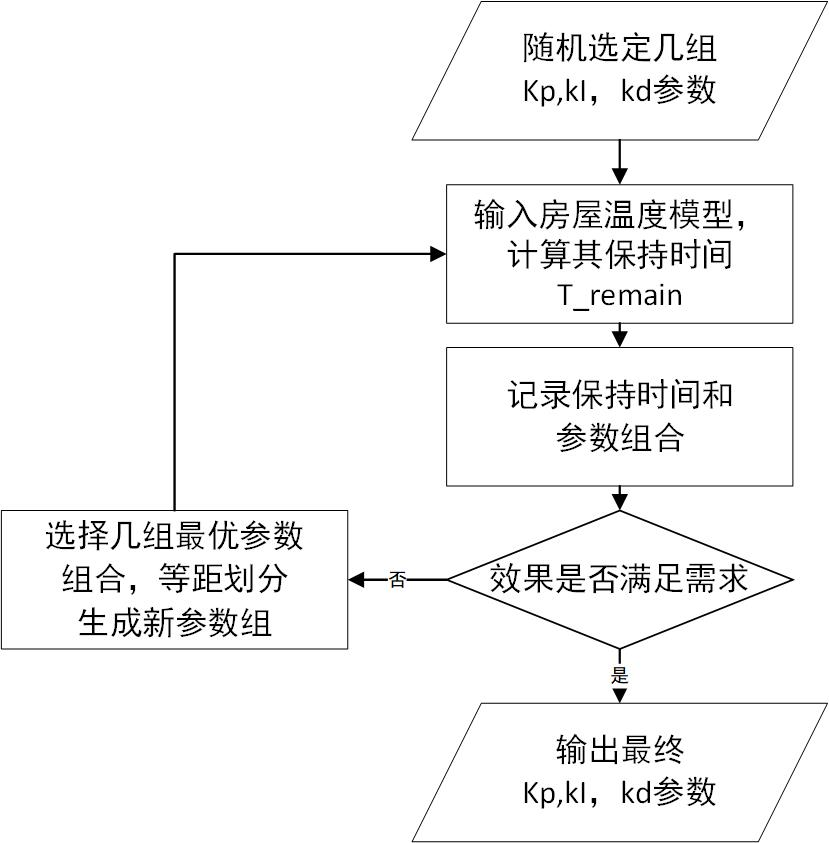
\includegraphics[width=0.7\textwidth]{liuc.jpg}
\caption{计算最优$K_p,K_i,K_d$参数的流程} % 标题
\label{five}
\end {figure}

\subsubsection{温度控制模型求解}

经过多次测试,我们选取参数组合$k_p = -0.01$,$k_i= 0.001$与$k_d = 0.05$进行24小时模拟,最终获得如下模拟结果:

\begin {figure}[h]
\centering % 居中显示
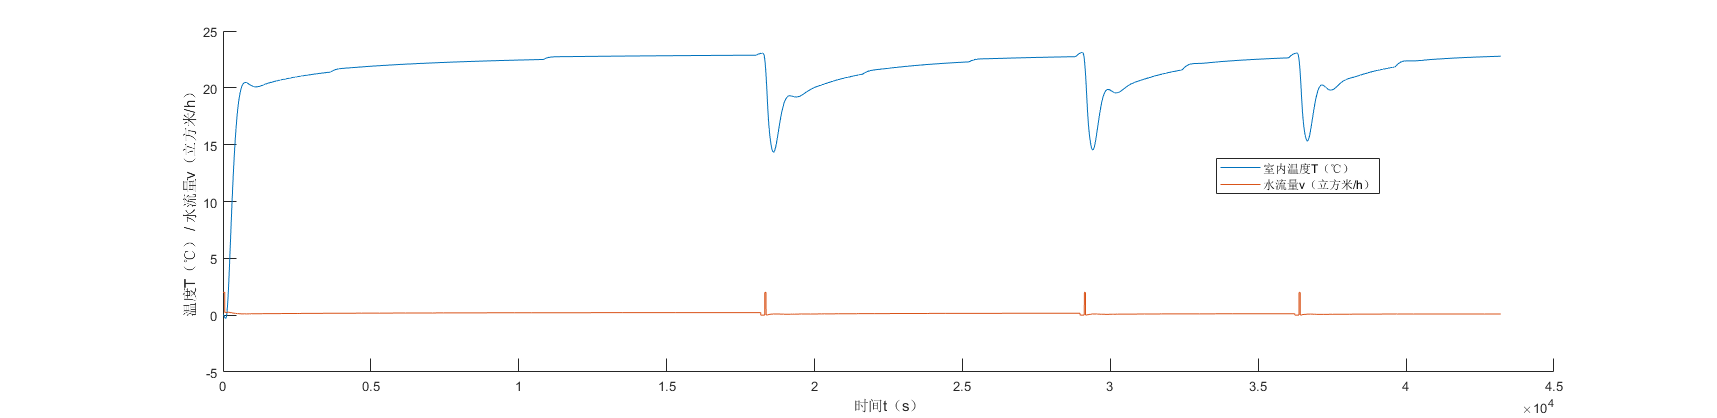
\includegraphics[width=\textwidth]{wd1.png}
 % 标题
\label{five}
\end {figure}
\begin {figure}[h]
\centering % 居中显示
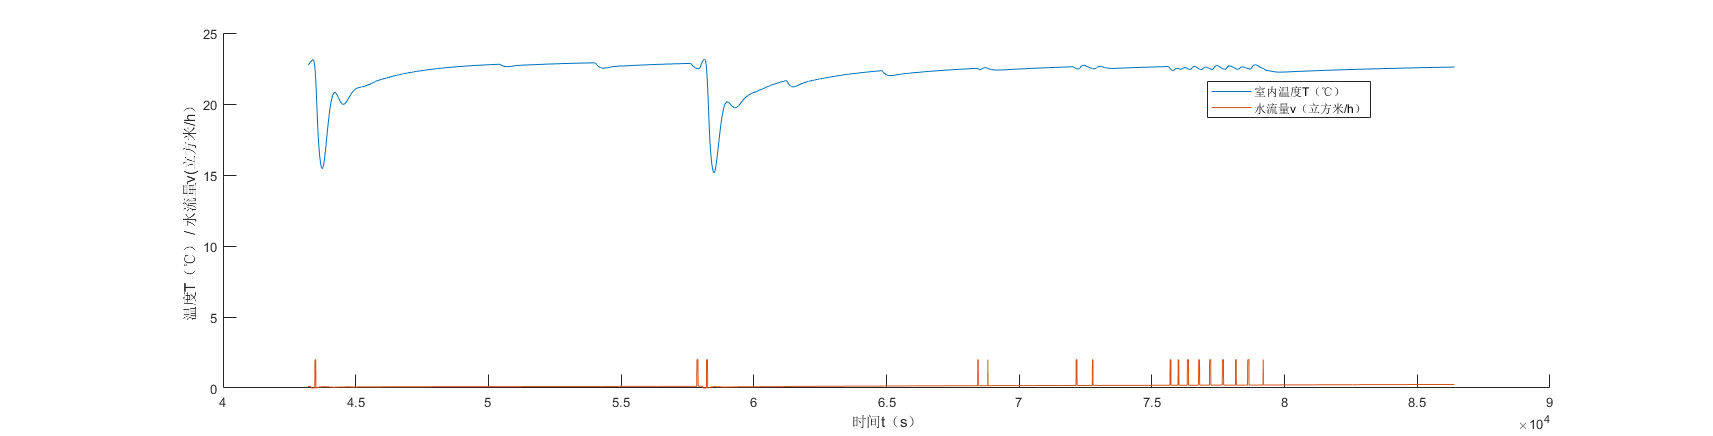
\includegraphics[width=\textwidth]{wd2.png}
\caption{PID控制下房间一日内的温度变化信息} % 标题
\label{five}
\end {figure}

可见在外界温度发生变化时,水流温度会做出调整,以维持室内温度保持一定范围之内,随后迅速恢复到设定的温度内。经过计算,在房屋温度从$0\degree C$开始,一直调控24小时的过程中,室内温度的均值为$21.86\degree C$方差为$1.753$,在24小时内,系统总共调节$1454$次。所得结果能基本完成题目要求,在时间和算力允许的条件下,可以找出更佳的参数组合取得更好效果。

由于该温控模型由室内温度变化来控制水流,没有对于房屋属性以及过去信息的记录,存在部分时间点温度波动过大的行为,我们将在下一小节进行改进。
\subsection{}
\section{六、敏感性分析}
\section{七、模型的评价}

\subsection{模型的优点}
\begin{enumerate}
    \item 采用

\end{enumerate}

\subsection{模型的缺点}
\begin{itemize}
    \item 利用较

\end{itemize}

%----------- 参考文献 ----------
\newpage
\bibliographystyle{unsrt} %规定了参考文献的格式
\begin{center}
\bibliography{reference} %调出LaTeX生成参考文献列表
\end{center}

%----------- 附录 ----------
\newpage
\section{附件}
\textbf{附件清单:}
\renewcommand\theenumi{\roman{enumi}}
% 规定数字格式为罗马数字
\renewcommand\labelenumi{\textbf{附录\theenumi}}
% 规定是附录某某
\begin{itemize}
    \item xxx代码
\end{itemize}

\textbf{sobel边缘检测代码}

\begin{lstlisting}[language=matlab]
    function GAdsa 
\end{lstlisting}



\end{document}